\documentclass[12pt,a4paper,onecolumn]{article}
\usepackage{covington}
\usepackage{comment}
\usepackage{url}
\usepackage{mathtools}
\usepackage{tipa}
\usepackage[UKenglish]{babel}
\usepackage{graphicx}
\usepackage{subfigure}

% Spaced paragraphs
\setlength{\parindent}{0.0in}
\setlength{\parskip}{0.1in}

% Default fixed font does not support bold face
\DeclareFixedFont{\ttb}{T1}{txtt}{bx}{n}{8} % for bold
\DeclareFixedFont{\ttm}{T1}{txtt}{m}{n}{8}  % for normal

% Custom colors
\usepackage{color}
\definecolor{deepblue}{rgb}{0,0,0.5}
\definecolor{deepred}{rgb}{0.6,0,0}
\definecolor{deepgreen}{rgb}{0,0.5,0}

\usepackage{listings}
\lstset{
language=Matlab,
basicstyle=\ttm,
breaklines=true,
otherkeywords={self},             % Add keywords here
keywordstyle=\ttb\color{deepblue},
emph={MyClass,__init__},          % Custom highlighting
emphstyle=\ttb\color{deepred},    % Custom highlighting style
stringstyle=\color{deepgreen},
frame=tb,                         % Any extra options here
showstringspaces=false  
}

\newcommand{\code}[2]{
  \hrulefill
  \subsection*{#1}
  \lstinputlisting{#2}
  \vspace{2em}
}


\begin{document}
\title{AV Assignment 2: 3D Image Analysis}
\author{s0949775 and s1330128}
\date{\today}
\maketitle


\section{Introduction}
This report covers the construction of a 3D model from a 
sequence of RGB and depth frames from the Kinect. 
The algorithms we chose and explored are discussed for
each phase of processing:
\begin{itemize}
\item Extracting the bin from the RGB images and corresponding 3D points.
\item Aligning the extracted bin points from each frame in a single coordinate frame.
\item Combining the aligned bin points into a single dataset.
\item Fitting planes to the sides of the bin.
\end{itemize}

\subsection{Box Extraction}
To extract the bin we used a series of techniques on the colour and depth data.  We first converted the image to a chromaticity image, and smoothed with a gaussian filter to reduce noise.  This accentuated the orange regions of the box and made them consistent throughout the sequence.  An example image from this stage is shown in figure \ref{fig:full_chromaticity_image}.

We manually thresholded the smoothed chromaticity image, using separate thresholds for each of the three colour channels, to detect the orange regions.  The output from this stage is shown in figure \ref{fig:thresholding_result}.

\begin{figure}[!ht]
    \centering
      \subfigure[RGB image converted to chromaticity coordinates and smoothed.]{
        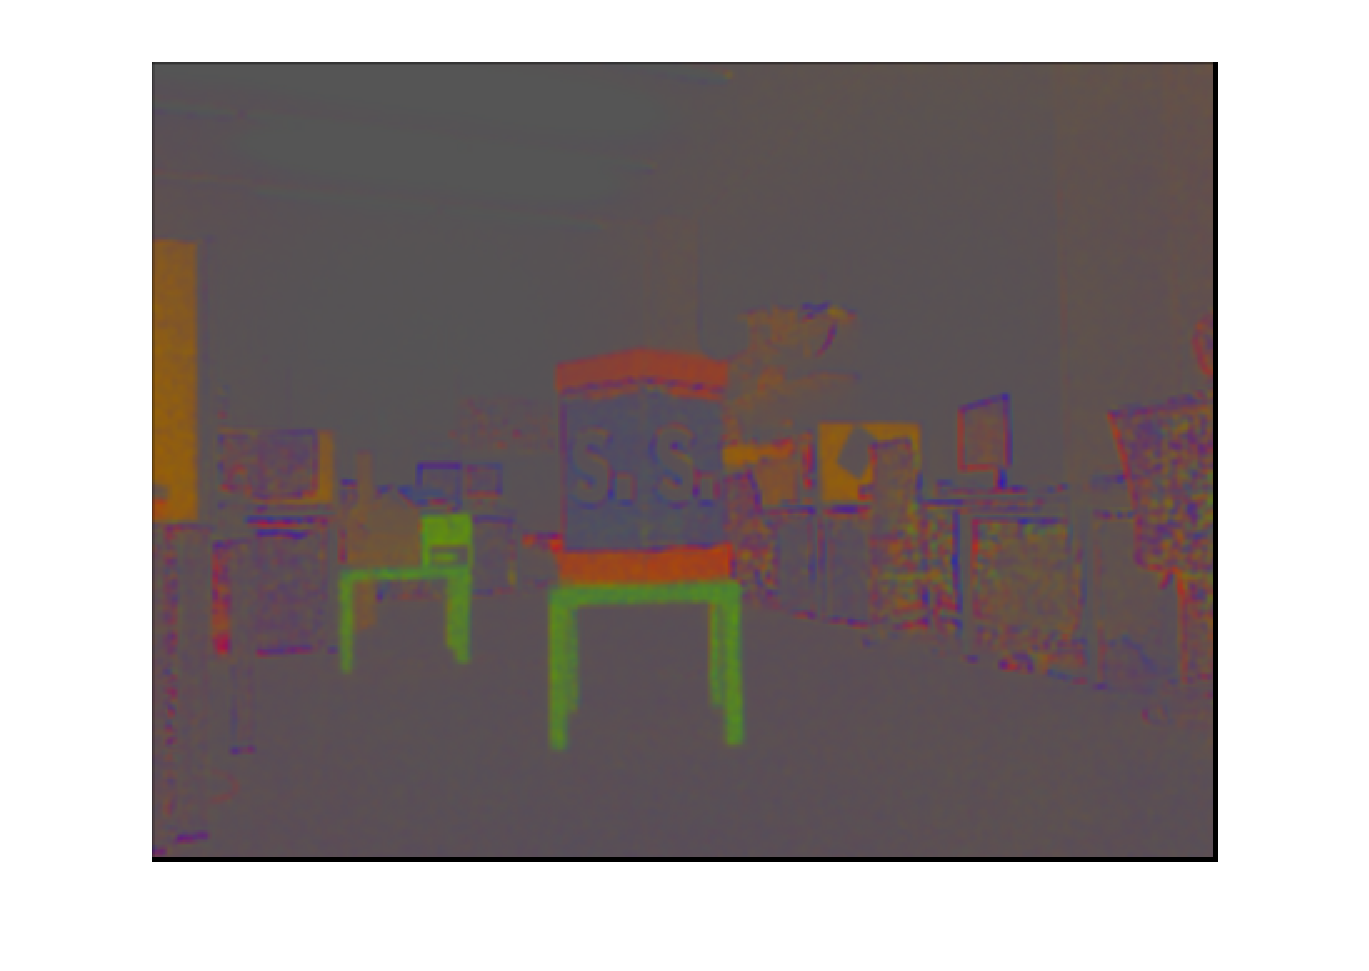
\includegraphics[width=0.45\linewidth]{figs/full_chromaticity_image}
        \label{fig:full_chromaticity_image}
      }
      \quad
      \subfigure[Thresholding colours to find orange regions.]{
        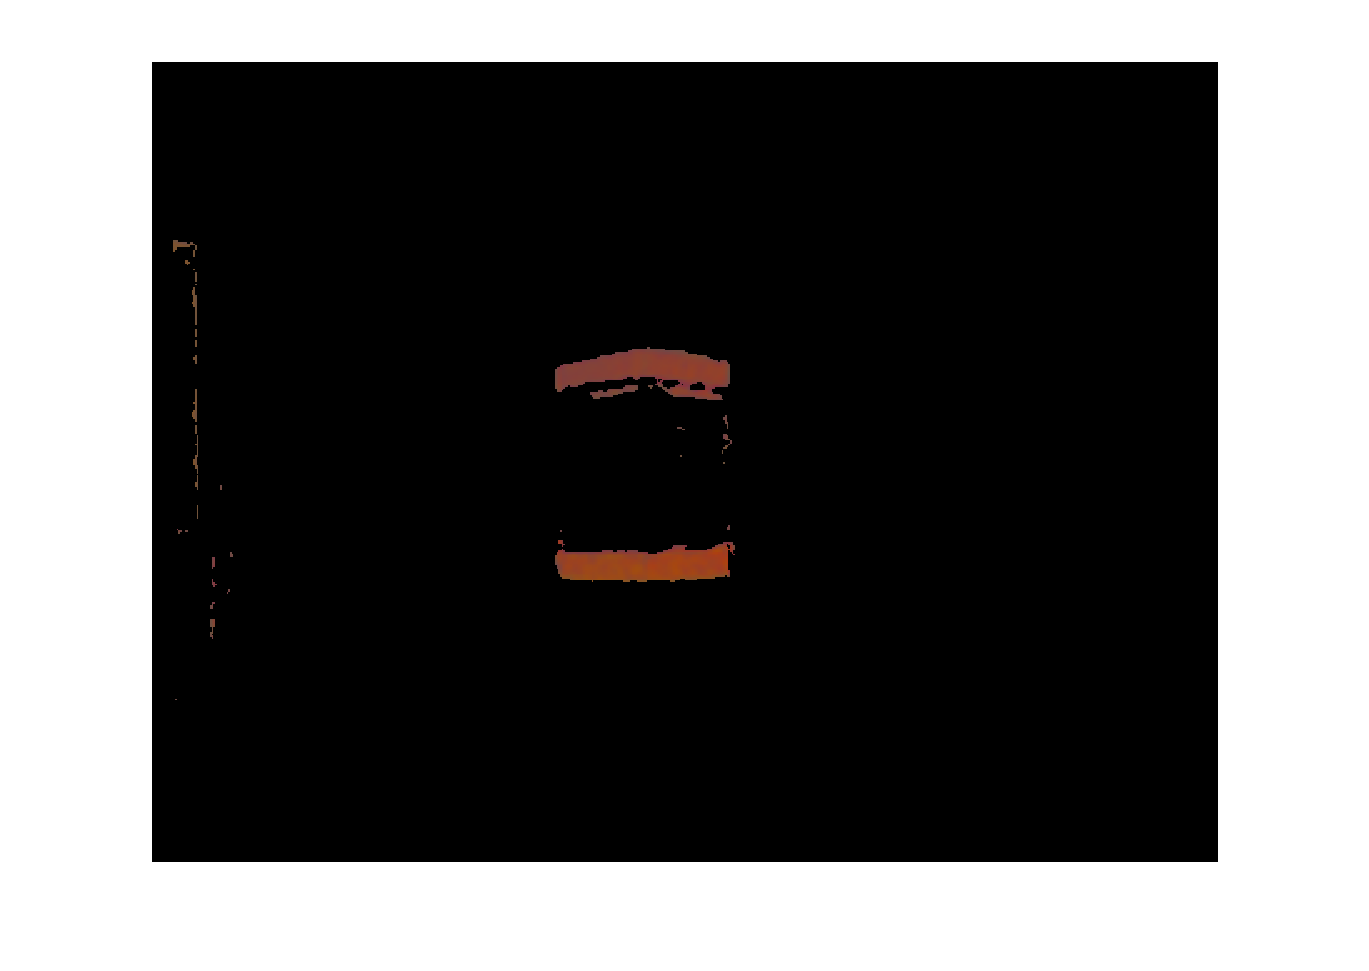
\includegraphics[width=0.45\linewidth]{figs/thresholding_result}
        \label{fig:thresholding_result}
      }

        \subfigure[Depth image.]{
        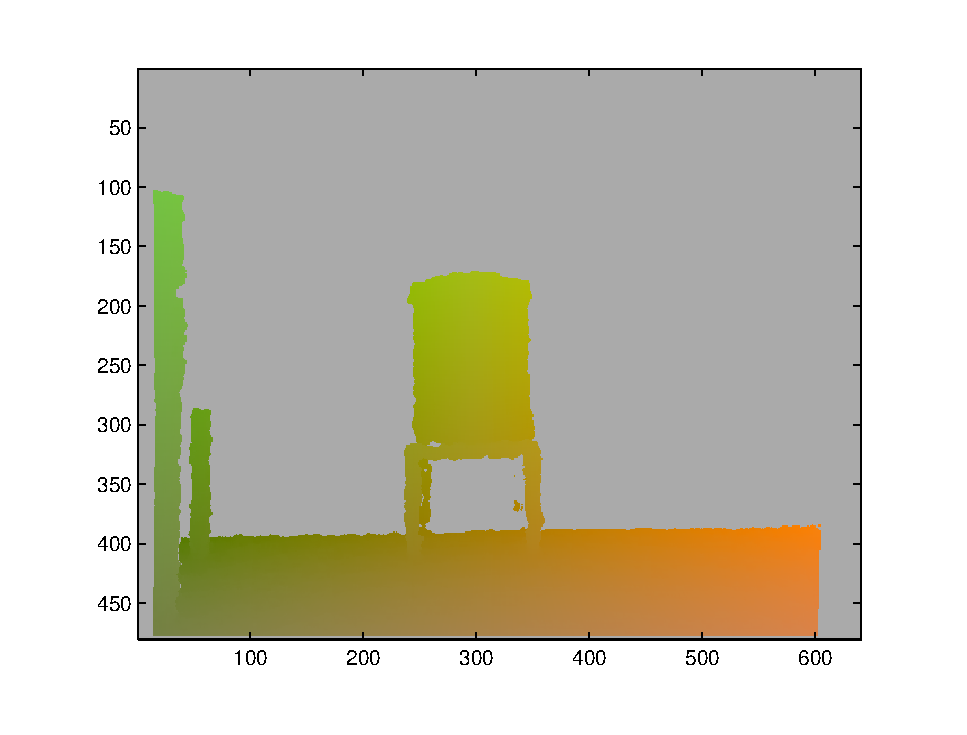
\includegraphics[width=0.45\linewidth]{figs/full_depth_data_picture}
        \label{fig:full_depth_data_picture}
      }
      \subfigure[Detected bottom of the bin.]{
        \includegraphics[width=0.45\linewidth]{figs/detected_bottom_orange_region_mask}
        \label{fig:detected_bottom_orange_region_mask}
      }
      \caption{Box extraction stages.}
\end{figure}

Some noise is present, which corresponds to other orange features in the scene.  To eliminate this, we took the intersection of the thresholded regions with the depth image (see figure \ref{fig:full_depth_data_picture}), and identified the two largest connected components remaining.  These corresponded to the orange regions at the top and bottom of the box.  From these we could reliably find the bottom of the box, as shown in figure \ref{fig:detected_bottom_orange_region_mask}.  Finally, to identify all of the pixels in the box, we took all pixels in the depth map that were above the bottom edge of the lower orange region, producing the image in figure \ref{fig:extracted_box_example}.

\begin{figure}[!ht]
  \centering
  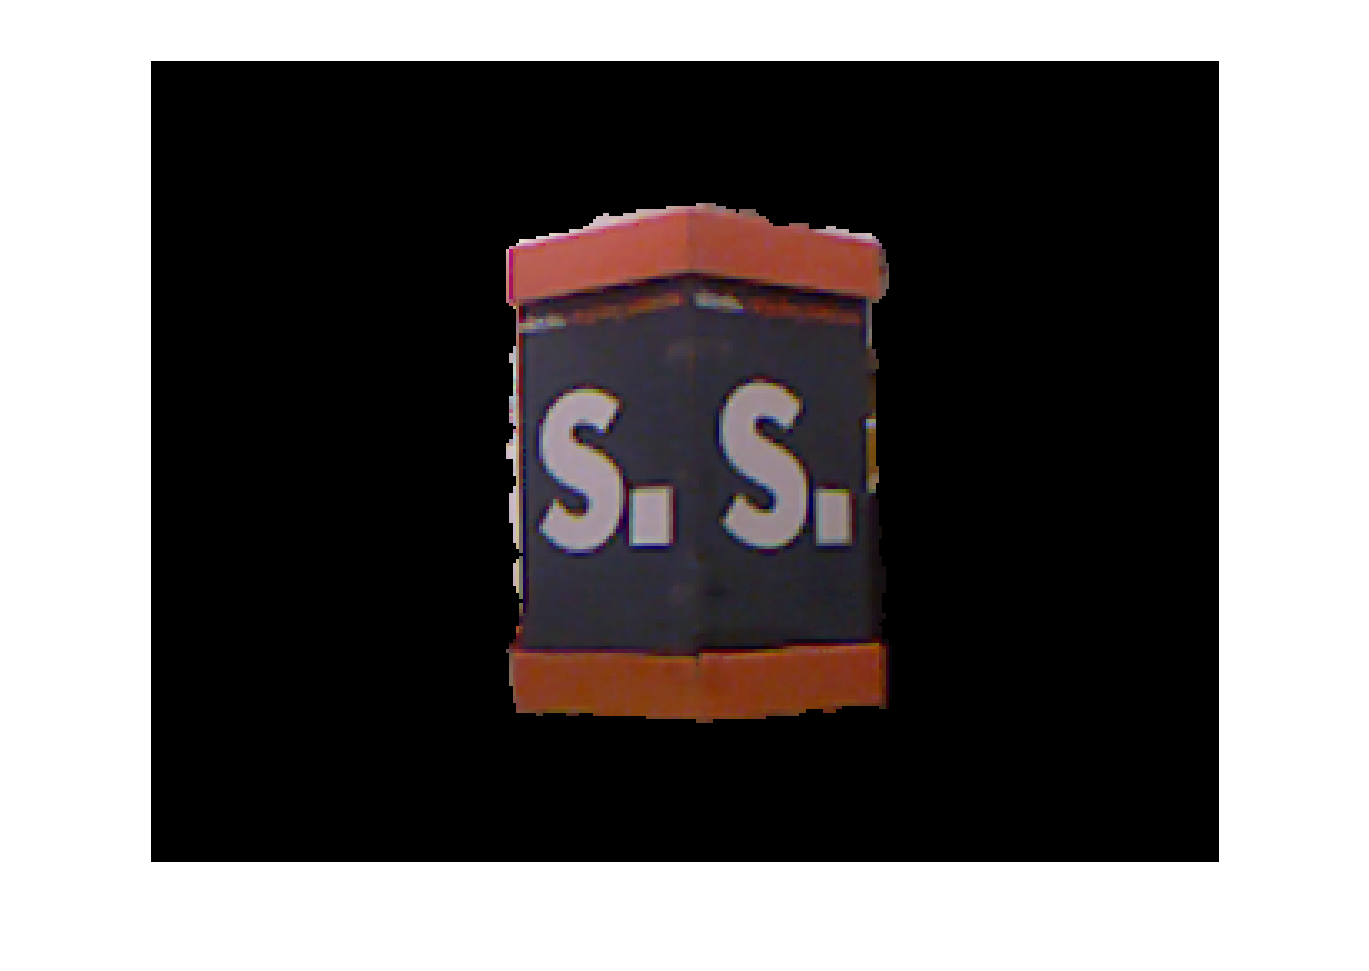
\includegraphics[width=1.0\textwidth]{figs/extracted_box_example}
  \caption{Final extracted box for one frame.}
  \label{fig:extracted_box_example}
\end{figure}

This technique worked well for the frames in the dataset, although it relied on knowledge specific to that dataset, such as the largest orange regions belonging to the box, and the box being isolated in the depth image.

The final image in figure \ref{fig:extracted_box_example} shows some noise around the box.  We tried removing this by using thresholds on the box pixels.  The noise could be removed quite effectively for individual frames, but no static threshold values worked over the whole sequence.  Adaptive thresholding could be used to deal with this, but we decided that the resulting box extraction was good enough for our purposes.



\begin{figure}[!ht]
    \centering
      \subfigure[Depth point data from single frame]{
        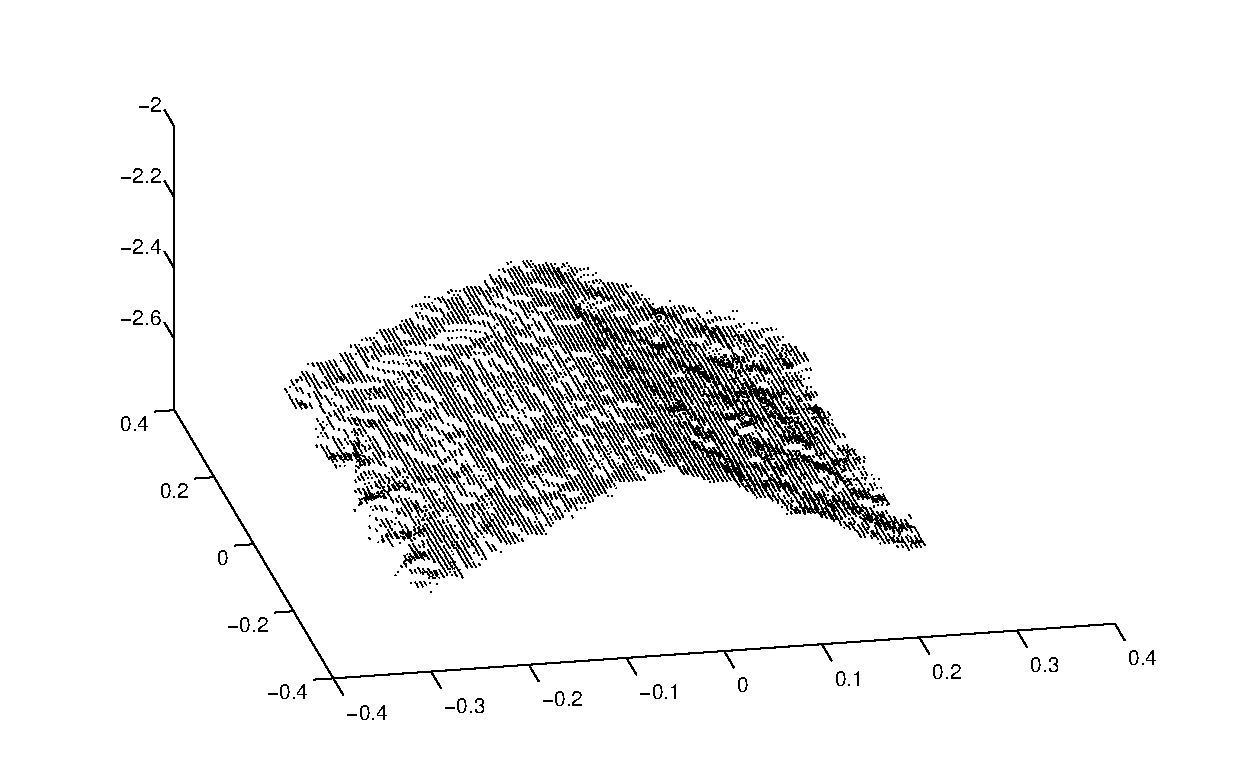
\includegraphics[width=0.475\linewidth]{figs/depth_points_example}
        \label{fig:depth_points_example}
      }
      \subfigure[Coloured depth points]{
        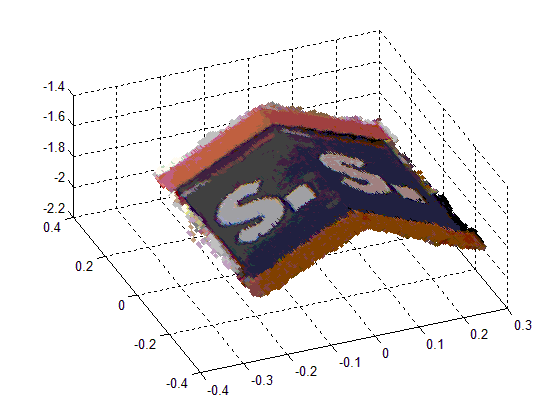
\includegraphics[width=0.475\linewidth]{figs/coloured_depth_points}
        \label{fig:coloured_depth_points}
      }
      \caption{Extracted box examples}
\end{figure}

\subsection{Point Alignment}
As was suggested in the assignment we took the middle frame
from the sequence as our foundation frame, against which we aligned all other frames.

To align points for different frames we used the ICP algorithm
linked to in the assignment.  Because the plane points are not very distinctive, we used the edge points for alignment.  We detected the edges using Canny edge detection on the extracted RGB box pixels, converted to greyscale.  We tuned the edge detector parameters to ensure that only the main edges of the box were detected, as in figure \ref{fig:extracted_edge_mask}.

\begin{figure}[!ht]
  \centering
  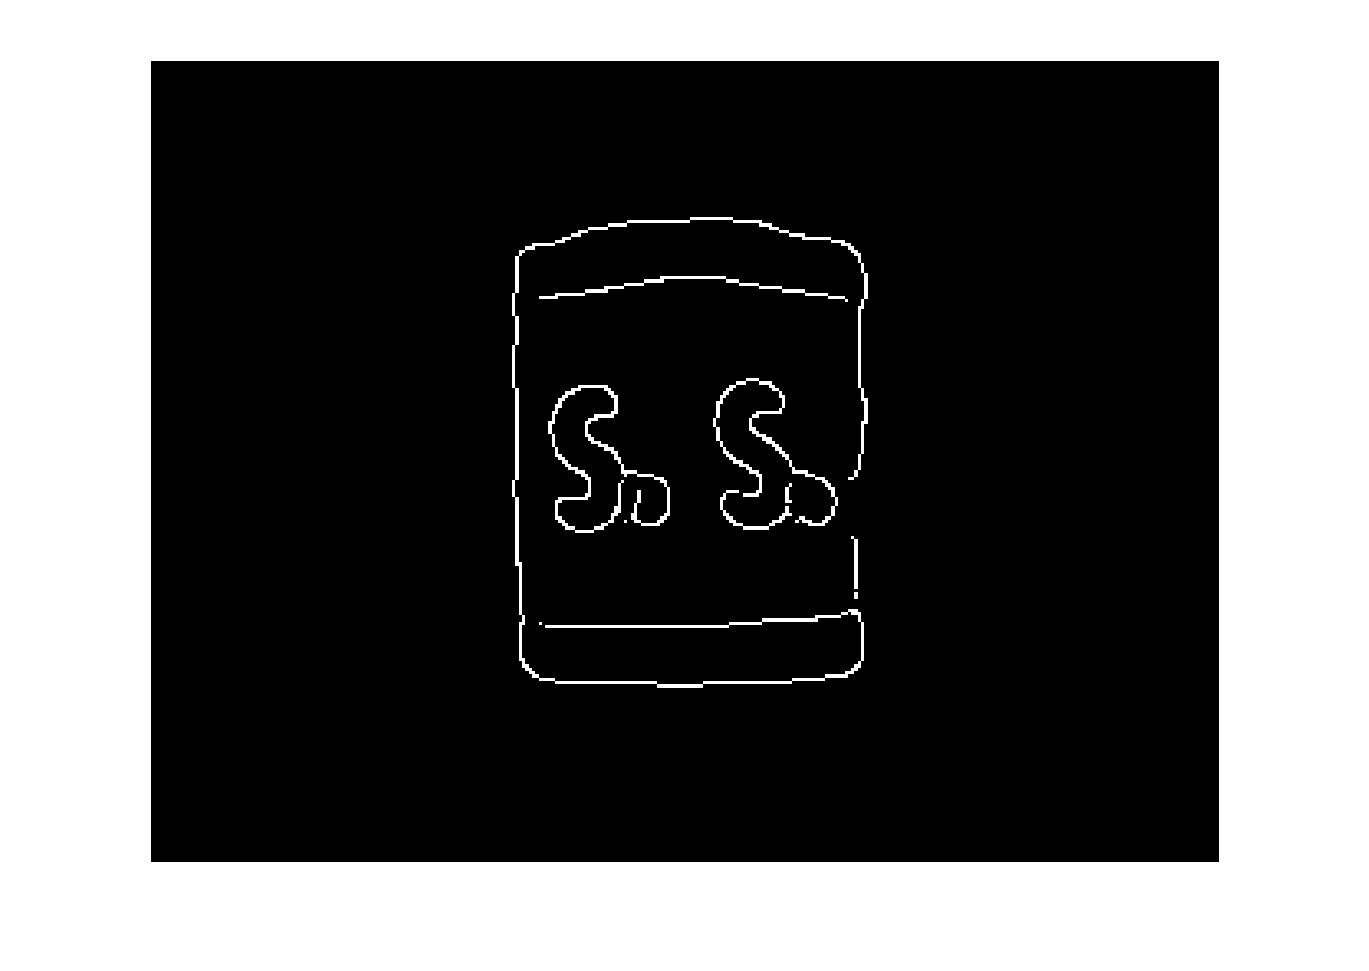
\includegraphics[width=0.5\textwidth]{figs/extracted_edge_mask}
  \caption{Extracted edges for ICP alignment}
  \label{fig:extracted_edge_mask}
\end{figure}

We took the 3D points corresponding to the detected greyscale edges and used them as input to the ICP algorithm.  Figures \ref{fig:icp_before_alignment_from_side} and\ref{fig:icp_before_alignment_from_top} show an example alignment from the top and the side.

\begin{figure}[!ht]
    \centering
      \subfigure[ICP alignment with edge points - top view]{
        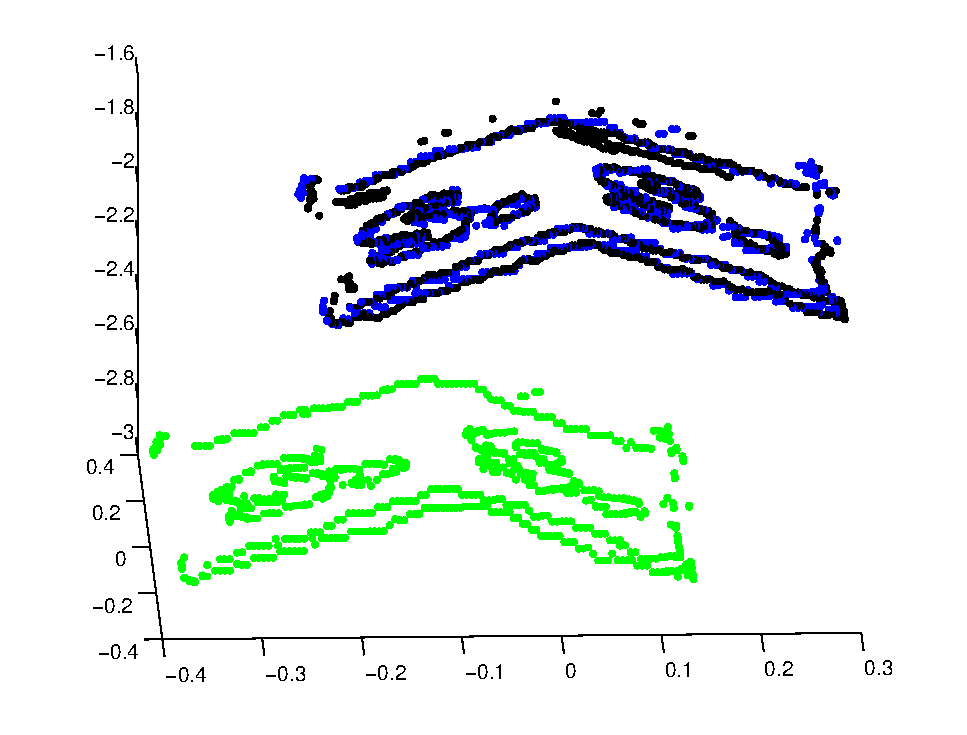
\includegraphics[width=0.475\linewidth]{figs/icp_before_alignment_from_side}
        \label{fig:icp_before_alignment_from_side}
      }
      \subfigure[ICP alignment with edge points - side view]{
        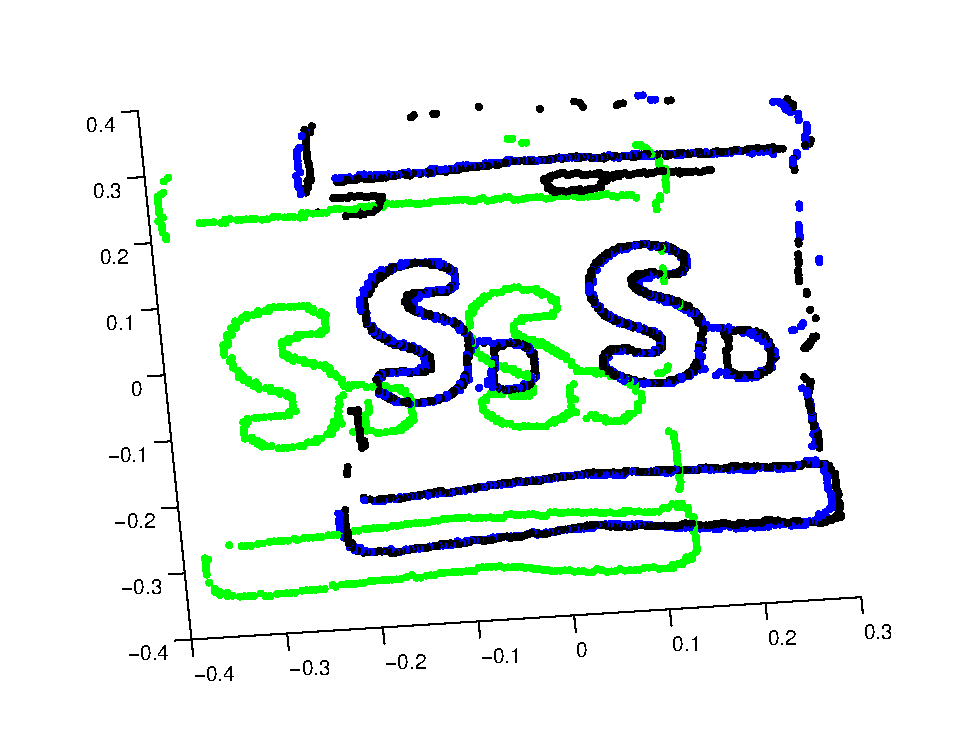
\includegraphics[width=0.475\linewidth]{figs/icp_before_alignment_from_top}
        \label{fig:icp_before_alignment_from_top}
      }
      \caption{ICP alignment.  The foundation frame is black.  The current frame is shown in green prior to alignment and blue after alignment.}
\end{figure}

We found that aligning with the edges alone produced good results, and we did not see an improvement when using all the points in the bin.  Figure \ref{fig:depth_points_after_edge_point_icp_alignment_ok} shows the results of an alignment with just edge points, while figure \ref{fig:depth_points_after_full_point_icp_alignment_ok} shows the alignment using a combined transformation from edge points and all the points.  There was no clear visual difference.  Using the edges alone was also much faster than using all the points.



\begin{figure}[!ht]	
    \centering
      \subfigure[Depth point alignment using ICP transformations estimated only with edge points]{
        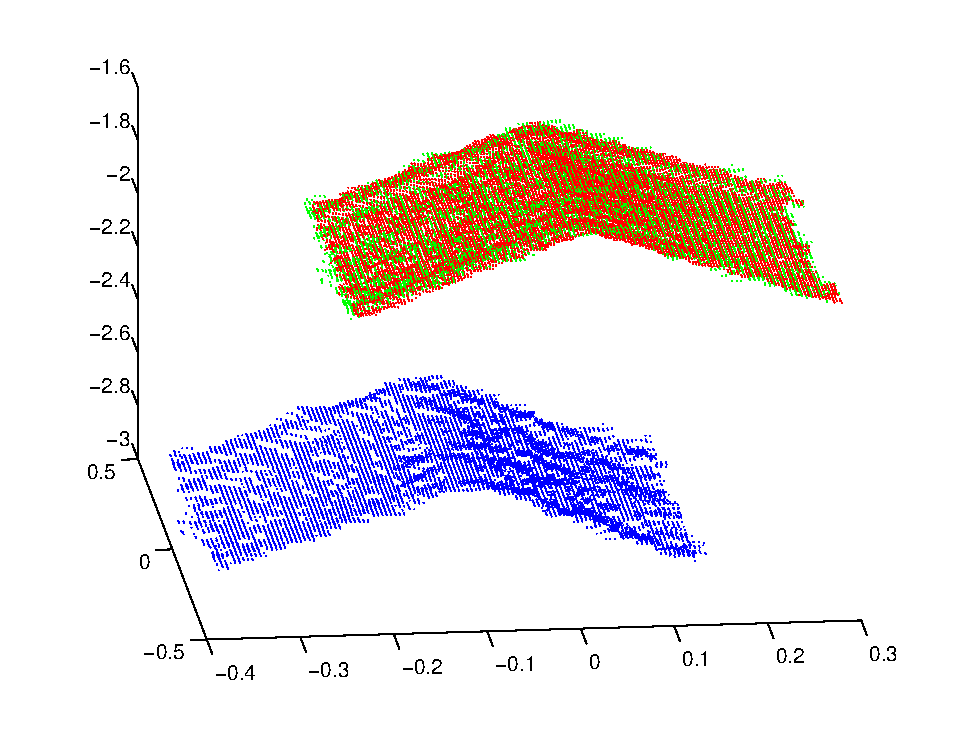
\includegraphics[width=0.475\linewidth]{figs/depth_points_after_edge_point_icp_alignment_ok}
        \label{fig:depth_points_after_edge_point_icp_alignment_ok}
      }
      \subfigure[Depth point alignment using ICP transformations estimated with 
      weighted edge points and full point set]{
        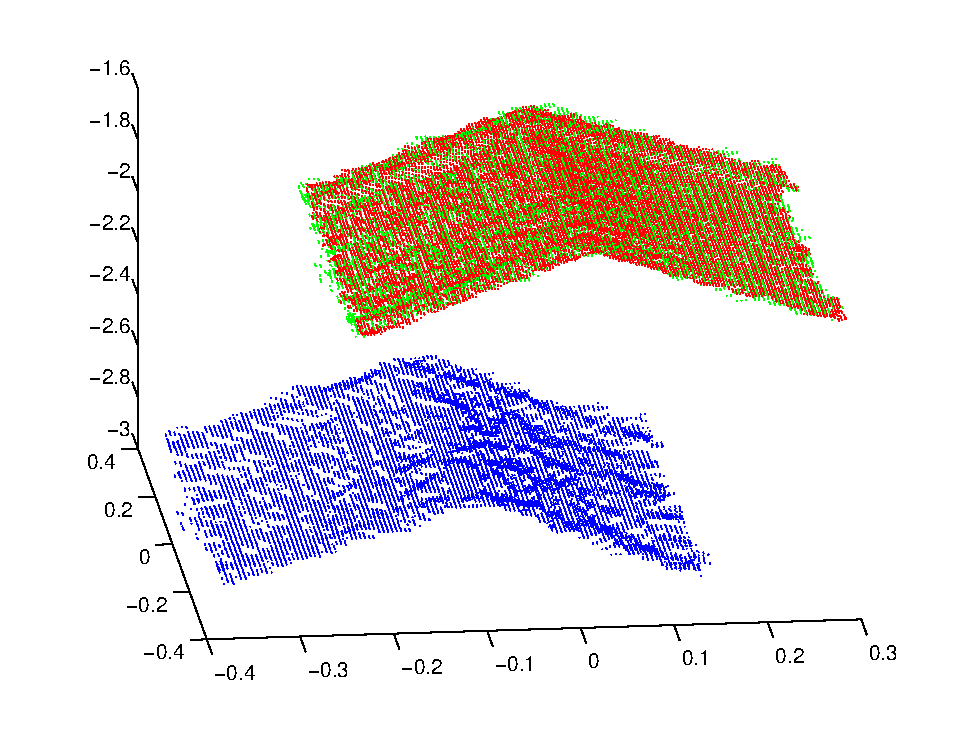
\includegraphics[width=0.475\linewidth]{figs/depth_points_after_full_point_icp_alignment_ok}
        \label{fig:depth_points_after_full_point_icp_alignment_ok}
      }
      \caption{Alignment of entire point dataset for the box. Red points are depth points from
      foundation frame, blue ones are from current frame for alignment and green ones (overlapping with red)
      are blue points after applying transformations estimated with ICP}
\end{figure}
\subsection{Plane Fitting}
For plane extraction we chose to implement modified K-means algorithm.
It uses plane's normal vector $\vec{n}$  and data point $ (x,y,z) $
dot product as a distance measure. In maximization step it refits
plane on assigned data points for each plane
 using SVD (as given in "fitplane.m"
algorithm"). Code can be found in appendix \ref{apen:code_in}.

This approach easily allowed to fit data points to any of number of
planes that was required though it is prone (as regular K-mean is)
to initialization. To cope with this, thresholds were introduced
to find cases when initialization was definitely wrong.


\begin{figure}[!ht]
    \centering
      \subfigure[Fitted planes]{
        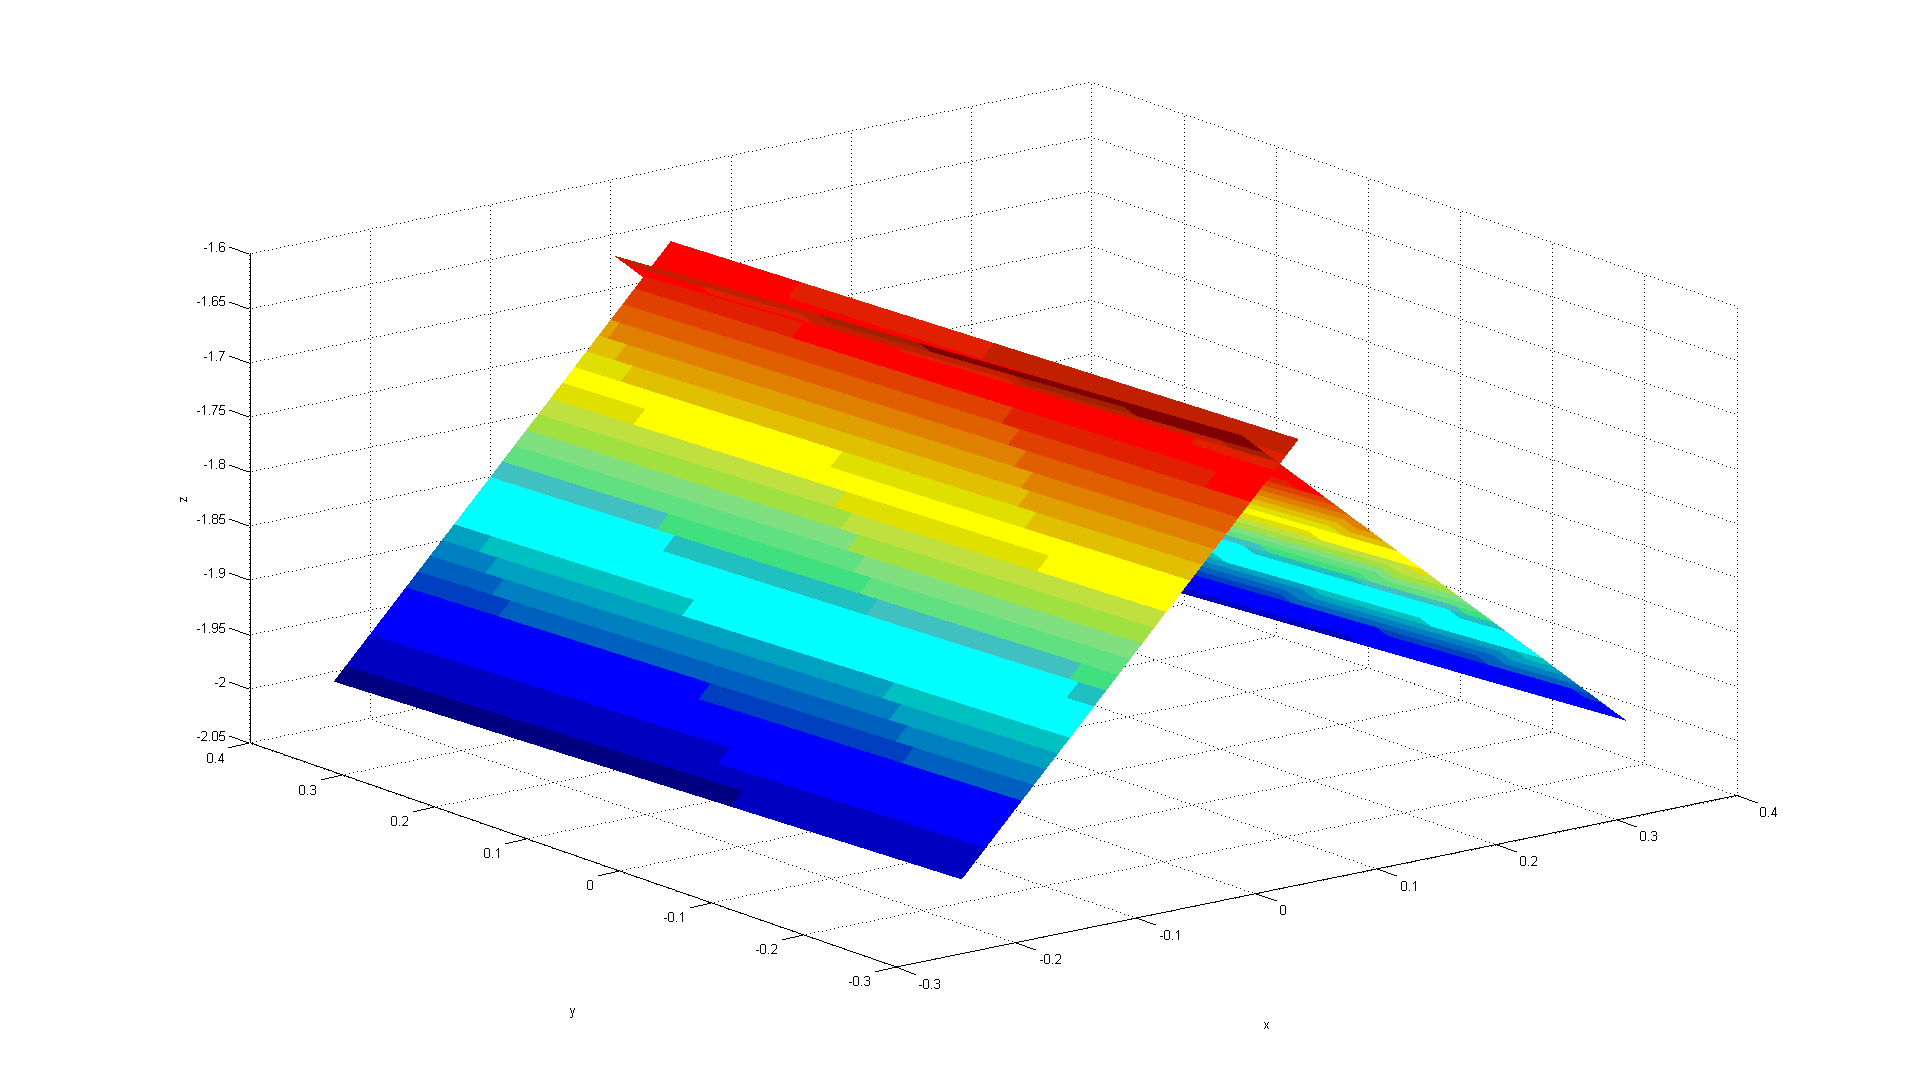
\includegraphics[width=0.475\linewidth]{figs/fitted_planes_without_points}
        \label{fig:fitted_planes_without_points}
      }
      \subfigure[Fitted planes together with final combined depth points]{
        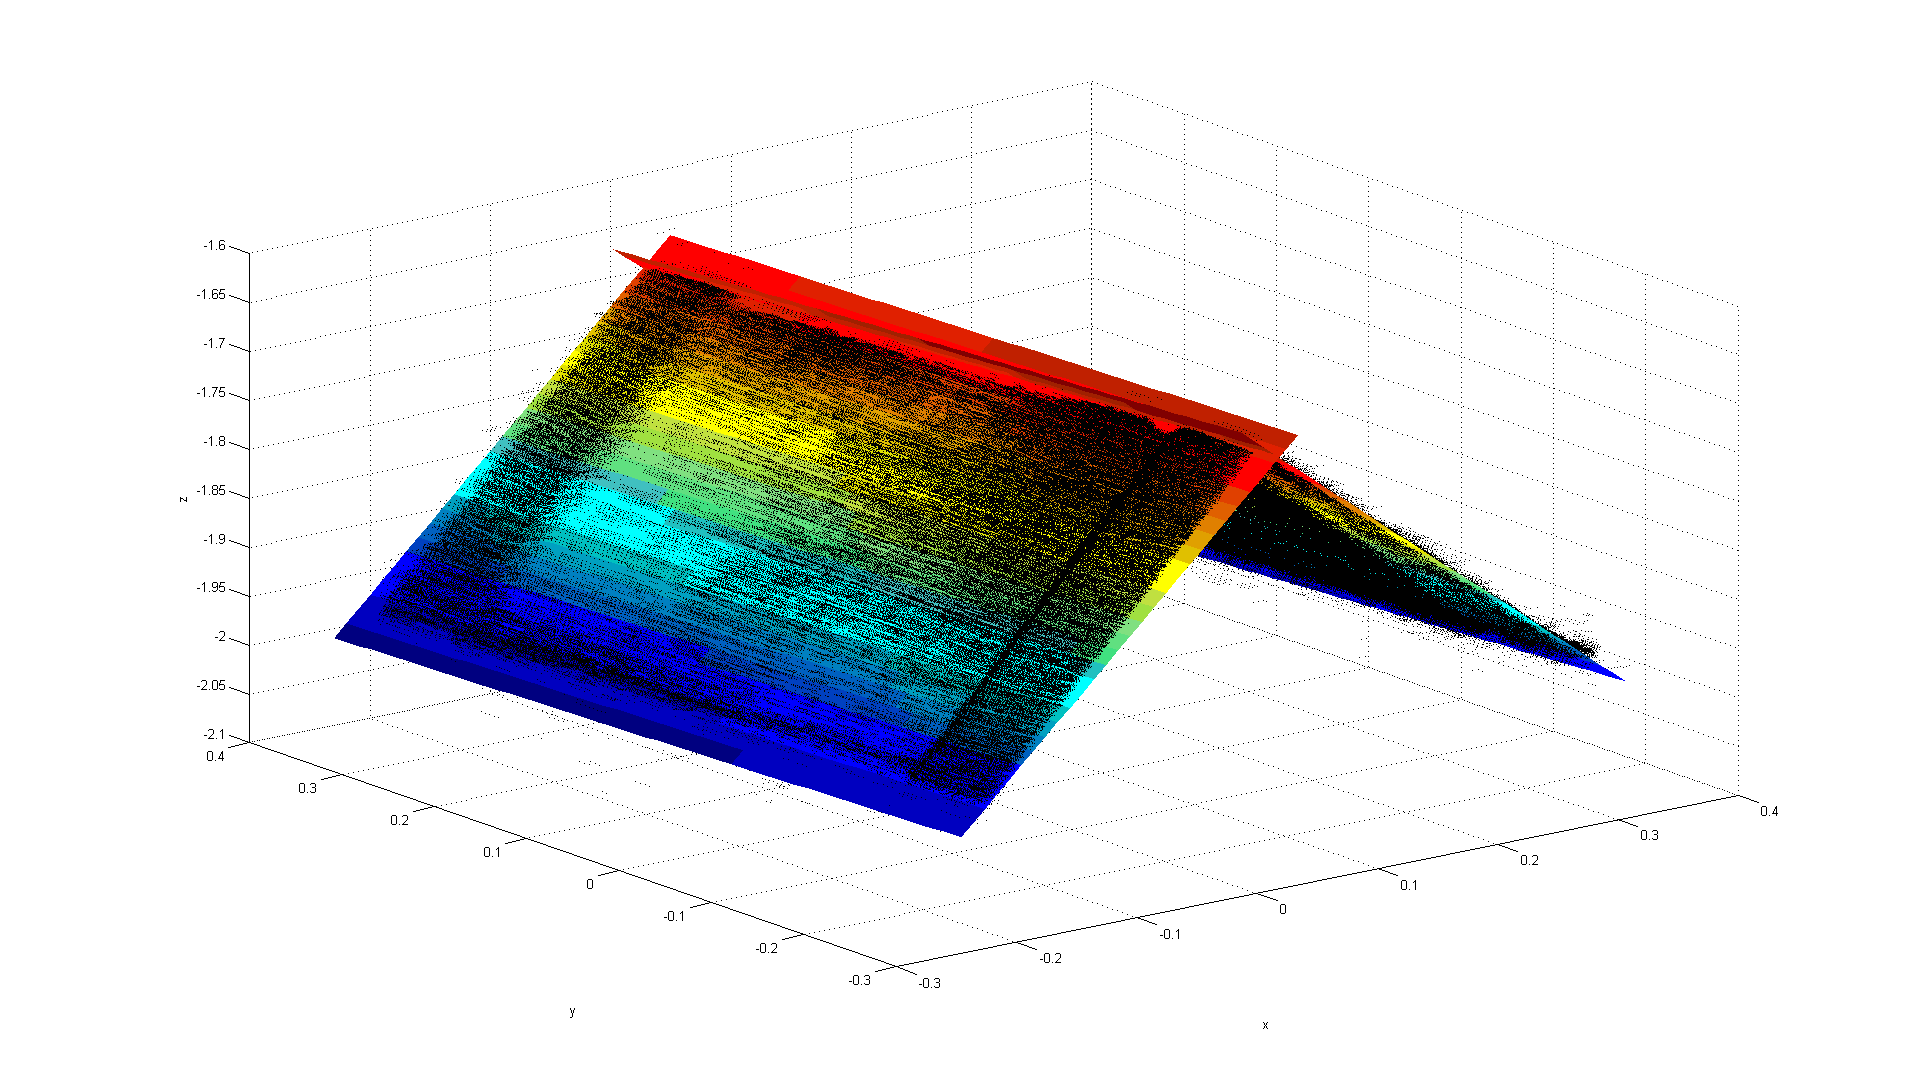
\includegraphics[width=0.475\linewidth]{figs/fitted_planes_with_points}
        \label{fig:fitted_planes_with_points}
      }
      \caption{Merged depth points shown together with fitted planes.}
\end{figure}
\section{Results}

\subsection{Dataset Merging}

\subsection{Alignment accuracy}
\begin{figure}[!ht]
  \centering
  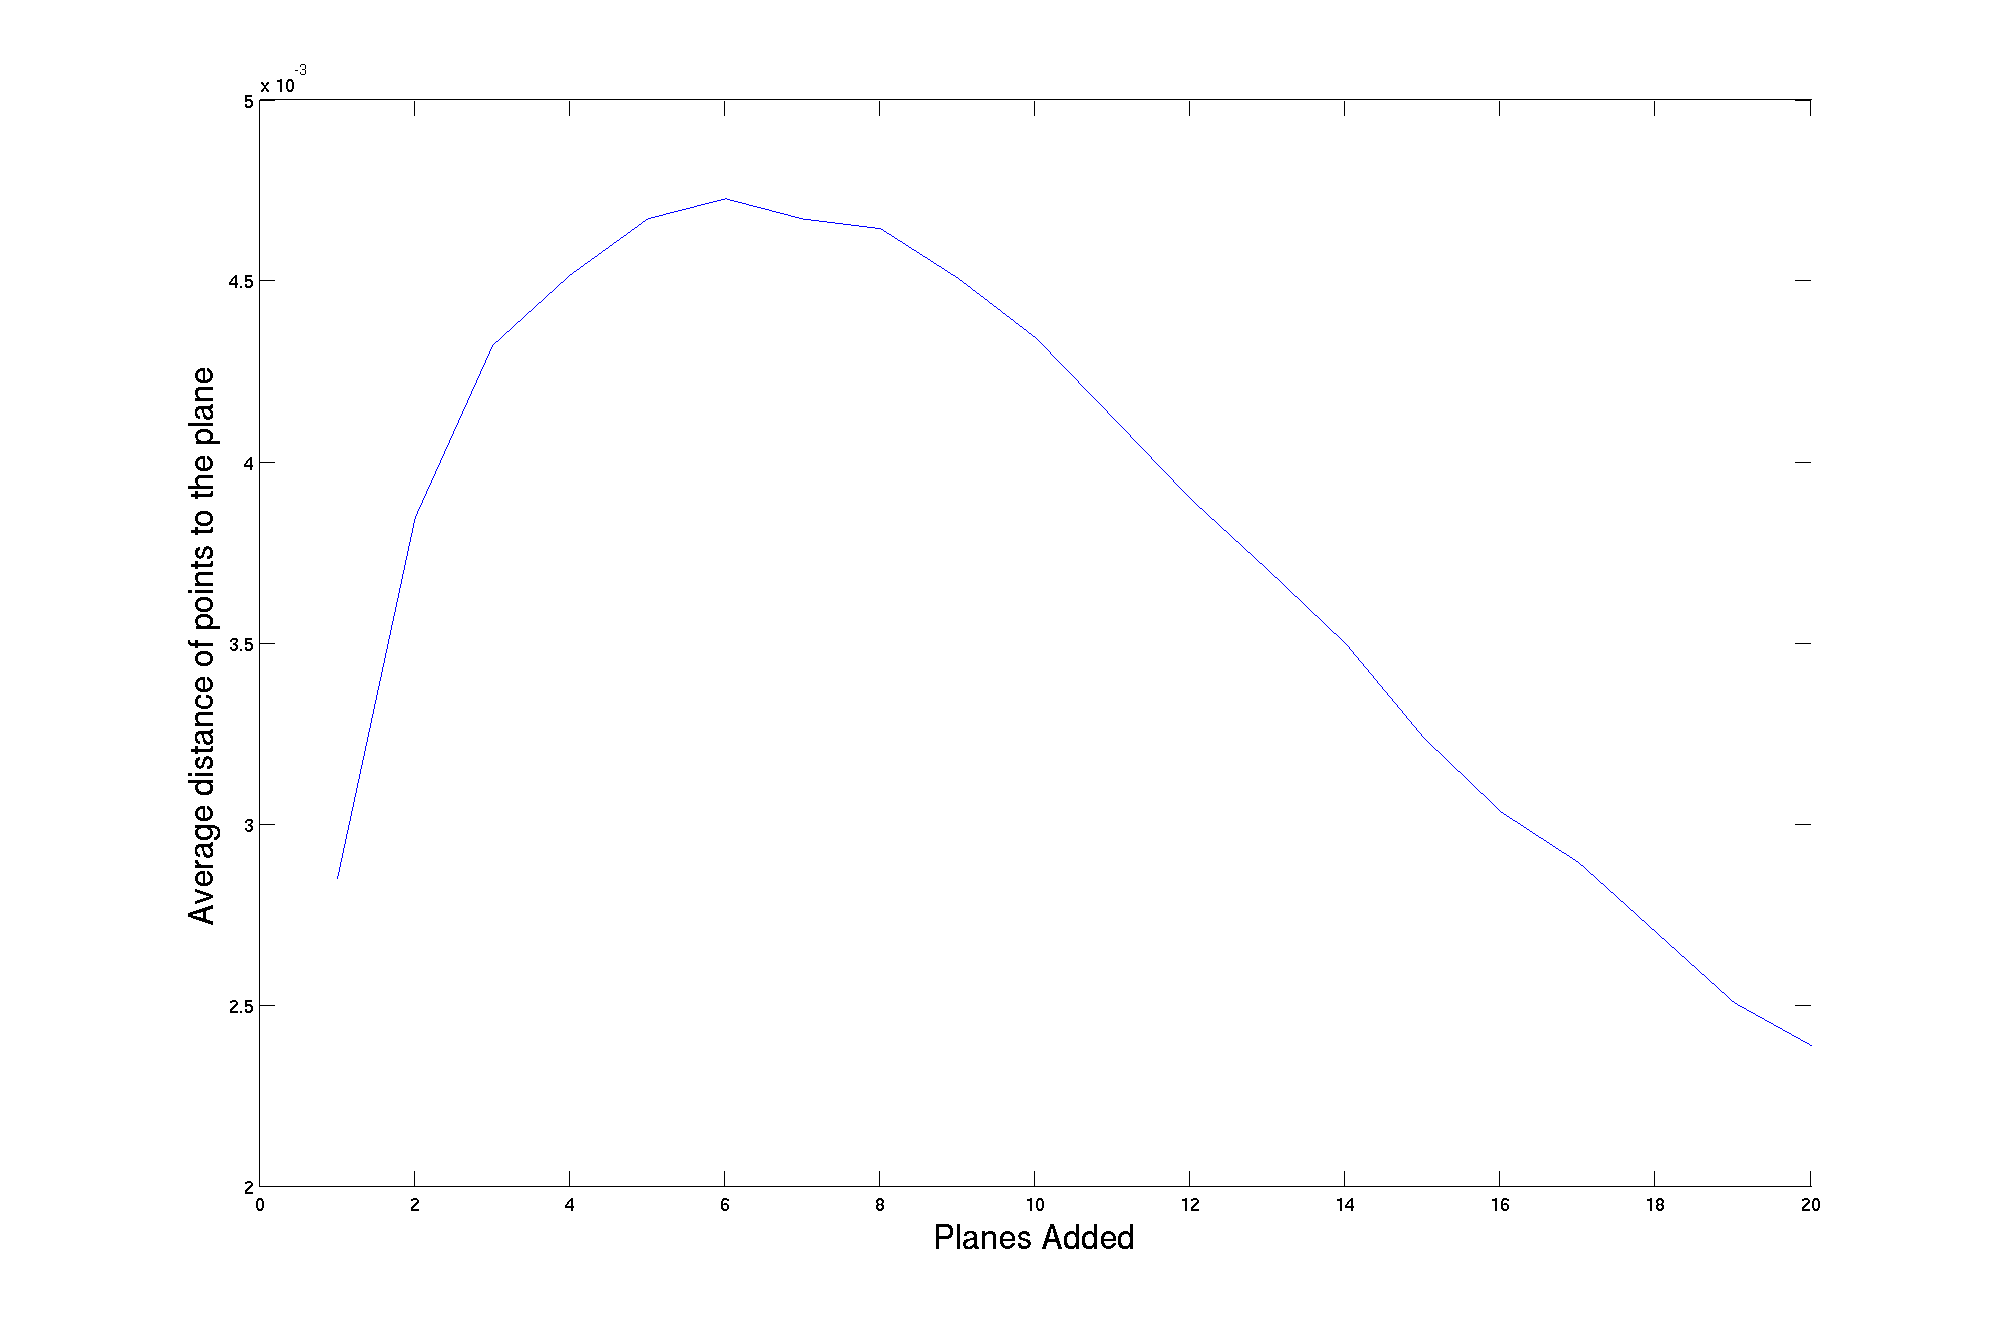
\includegraphics[width=0.5\textwidth]{figs/plane_angle_error_versus_foundation_plane}
  \caption{Dependency of frames combinedd and absolute mean distance of every point in "S." region to the plane}
  \label{fig:plane_angle_error_versus_foundation_plane}
\end{figure}
\subsection{Plane fitting}

\section{Discussion}
ICP and plane fitting algorithms in most cases 
worked without problems. K-means sometimes suffered
from poor initialization but that is easy to 
fix giving just a few checks of total
absolute error. The trickiest part is initial box
region detection. Finetuning color thresholds is tedious
process and always captures some artefacts around the box
that might have impact in later stages.

One of possible techniques to try for box detection
would be a probabilistic modelling - it might be possible
to detect background from whole series of frames
and then use it on each frame individually. 
We haven't tried this and just sticked with
easy to implement approach that works good enough.

\begin{thebibliography}{9}
  
\bibitem{lecture_code}
  ADVANCED VISION - TASK 4 MATLAB CODE
  \url{http://www.inf.ed.ac.uk/teaching/courses/av/MATLAB/TASK4/} 
  
\end{thebibliography}

\appendix


\newpage



\newpage
\section{Code}
\label{apen:code_in}

%\lstinputlisting[caption=assgn\_tracking.m, language=Matlab]{../assgn_tracking.m}




\end{document}
